\section{Hệ thức lượng trong tam giác}

\subsection{Đề 1}
\Opensolutionfile{ans}[ans/ans-0-C3B2.D1]
\caulc
\begin{ex}%[0H4N2-2]
	Cho $\Delta ABC$ có $a=4$, $c=5$, $\widehat{B}=150^\circ$. Tính diện tích tam giác $ABC$.
	\choice
	{$S=10$}
	{$S=10\sqrt{3}$}
	{\True $S=5$}
	{$S=5\sqrt{3}$}
	\loigiai{
		Diện tích tam giác $ABC$ là $S=\dfrac{1}{2}ac\sin \widehat{B}=\dfrac{1}{2}\cdot 4\cdot 5\sin 150^\circ =5$.}
\end{ex}
\begin{ex}%[0H4N2-2]
	Cho $\triangle ABC$ có $a=2$; $b=6$; $\widehat{C}=135^\circ $. Diện tích của tam giác là
	\choice
	{$6\sqrt{2}$}
	{\True $3\sqrt{2}$}
	{$4\sqrt{3}$}
	{$4$}
	\loigiai{
		Ta có $S=\dfrac{1}{2}a\cdot b\cdot\sin C=\dfrac{1}{2}\cdot 2\cdot 6\cdot sin135^\circ =3\sqrt{2}$.}
\end{ex}
\begin{ex}%[0H4N2-2]
	Cho tam giác $ABC$ có $\widehat{A}=60^\circ$, $b=10$, $c=20$. Diện tích tam giác $ABC$ bằng
	\choice
	{$70\sqrt{3}$}
	{$60\sqrt{3}$}
	{\True $50\sqrt{3}$}
	{$40\sqrt{3}$}
	\loigiai{
		Ta có $S_{\triangle ABC}=\dfrac{1}{2}b\cdot c\cdot \sin \widehat{A}=\dfrac{1}{2}\cdot 10\cdot 20\cdot \sin 60^\circ =50\sqrt{3}$.}
\end{ex}
\begin{ex}%[0H4N2-2]
	Cho $\triangle ABC$ có $a=2$, $b=6$, $\widehat{C}=153^\circ$. Diện tích của tam giác là
	\choice
	{$4$}
	{$6\sqrt{2}$}
	{\True $3\sqrt{2}$}
	{$4\sqrt{2}$}
	\loigiai{
		Ta có $S_{\triangle ABC}=\dfrac{1}{2}a\cdot b\cdot\sin C=\dfrac{1}{2}\cdot 2\cdot 6\cdot\sin{135^\circ}=3\sqrt{2}$.}
\end{ex}
\begin{ex}%[0H4N2-2]
	Tam giác có độ dài ba cạnh lần lượt là $9$, $10$, $11$ có diện tích bằng
	\choice
	{$15\sqrt{2}$}
	{\True $30\sqrt{2}$}
	{$50\sqrt{3}$}
	{$25\sqrt{3}$}
	\loigiai{
		Nửa chu vi của tam giác đã cho là $p=\dfrac{9+10+11}{2}=15$.\\
		Diện tích của tam giác đã cho là $S=\sqrt{p\left(p-9\right)\left(p-10\right)\left(p-11\right)}=30\sqrt{2}$.}
\end{ex}
\begin{ex}%[0H4V3-2]
	Khoảng cách từ $A$ đến $B$ không thể đo trực tiếp được vì phải qua một đầm lầy. Người ta xác định được một điểm $C$ mà từ đó có thể nhìn được $A$ và $B$ dưới một góc $60^\circ $. Biết $CA=200~\left(\mathrm{m}\right)$, $CB=180~\left(\mathrm{m}\right)$. Khoảng cách $AB$ bằng bao nhiêu?
	\choice
	{$168~\left(\mathrm{m}\right)$}
	{$228~\left(\mathrm{m}\right)$}
	{\True $20\sqrt{91}~\left(\mathrm{m}\right)$}
	{$112~\left(\mathrm{m}\right)$}
	\loigiai{
		\begin{center}
			{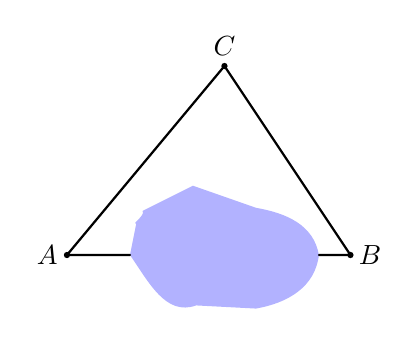
\begin{tikzpicture}[line join=round, line cap=round,>=stealth,thick,scale=0.8]
					%	\draw plot[smooth,tension=0.7,blue] coordinates{(0,0) (1,-1) (2,-0.8) (3,0) (2,1.3) (1,1) (0.2,0.7) (0,0)};
					\fill[blue!30] (0,0)
					to[out=-55,in=200] (1.05,-0.8)--(2,-.85)
					to[out=10,in=263] (3,0)
					to[out=100,in=-10] (2,0.75)--(1,1.1)--(0.2,0.7)
					to[out=-55,in=190] (.1,0.5)--cycle;
					\path
					(-1,0) coordinate (A)
					(1.5,3) coordinate (C)
					(3.5,0) coordinate (B);
					\draw [thick] (0,0)--(A)--(C)--(B)--(3,0);
					\foreach \i/\g in {C/90, A/180, B/0} \fill (\i)circle(.05) node[shift={(\g:.25)}] {$\i$};
			\end{tikzpicture}}
		\end{center}
		$AB^2=CA^2+CB^2-2CA\cdot CB\cdot\cos 60^\circ =36400$ $\Rightarrow AB=20\sqrt{91}~\left(\mathrm{m}\right)$.}
\end{ex}
\begin{ex}%[0H4H2-1]
	Khoảng cách từ $A$ đến $B$ không thể đo trực tiếp được vì phải đi qua một đầm lầy. Người ta xác định một điểm $C$ mà từ đó có thể nhìn được $A$ và $B$ dưới một góc $78^\circ 24'$. Biết rằng $CA=250\mathrm{~m}$, $CB=120\mathrm{~m}$. Khoảng cách $AB$ bằng bao nhiêu?
	\choice
	{\True $255\mathrm{~m}$}
	{$166\mathrm{~m}$}
	{$298\mathrm{~m}$}
	{$266\mathrm{~m}$}
	\loigiai{
		Ta có $AB=\sqrt{AC^2+BC^2-2AC\cdot BC\cdot\cos \widehat{ACB}}\approx 255\mathrm{~m}$.}
\end{ex}
\begin{ex}%[0H4V3-2]
	Khoảng cách từ $A$ đến $C$ không thể đo trực tiếp vì phải qua một đầm lầy nên người ta làm như sau. Xác định một điểm $B$ có khoảng cách $AB$ là $12\mathrm{~km}$ và đo được góc $\widehat{ACB}=37^\circ $. Hãy tính khoảng cách $AC$ biết rằng $BC$ bằng $5\mathrm{~km}$.
	\choice
	{$AC\approx 17\mathrm{~km}$}
	{$AC\approx 12\mathrm{~km}$}
	{\True $AC\approx 15{,}6 \mathrm{~km}$}
	{$AC\approx 20 \mathrm{~km}$}
	\loigiai{
		\begin{center}
			\begin{center}
				{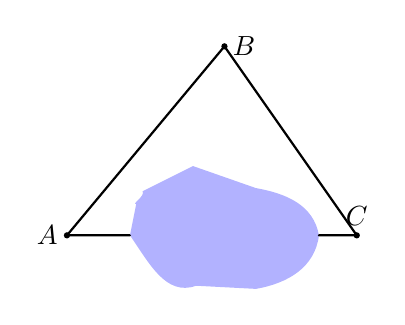
\begin{tikzpicture}[line join=round, line cap=round,>=stealth,thick,scale=0.8]
						%	\draw plot[smooth,tension=0.7,blue] coordinates{(0,0) (1,-1) (2,-0.8) (3,0) (2,1.3) (1,1) (0.2,0.7) (0,0)};
						\fill[blue!30] (0,0)
						to[out=-55,in=200] (1.05,-0.8)--(2,-.85)
						to[out=10,in=263] (3,0)
						to[out=100,in=-10] (2,0.75)--(1,1.1)--(0.2,0.7)
						to[out=-55,in=190] (.1,0.5)--cycle;
						\path
						(-1,0) coordinate (A)
						(1.5,3) coordinate (B)
						(3.6,0) coordinate (C);
						\draw [thick] (0,0)--(A)--(B)--(C)--(3,0);
						\foreach \i/\g in {C/90, A/180, B/0} \fill (\i)circle(.05) node[shift={(\g:.25)}] {$\i$};
				\end{tikzpicture}}
			\end{center}
		\end{center}
		Áp dụng đinh lí Côsin ta có 
		\begin{eqnarray*}
			&&AB^2=AC^2+BC^2-2AC\cdot BC\cdot \cos \widehat{ACB}\\
			&\Leftrightarrow& 144=AC^2+25-10\cdot AC\cdot \cos 37^\circ\\
			&\Leftrightarrow& AC^2-10\cdot AC\cdot \cos 37^\circ -119=0\\
			&\Leftrightarrow& \hoac{&AC=5\cos 37^\circ +\sqrt{25\cos^237^\circ +119}\approx 15{,}6&& (\text{nhận}) \\&AC=5\cos 37^\circ -\sqrt{25\cos^237^\circ +119}\approx -7{,}6. &&(\text{loại})}
		\end{eqnarray*}
		Vậy $AC\approx 15{,}6 \mathrm{~km}$.}
\end{ex}
\begin{ex}%[0H4V3-2]
	\immini{Để đo khoảng cách từ một ngôi nhà ven hồ đến một hòn đảo nhỏ giữa hồ, người ta chọn một gốc cây (trên bờ hồ) cách ngôi nhà $50$ m và gọi vị trí ngôi nhà là điểm $A$, gốc cây là điểm $B$, hòn đảo là điểm $C$, người ta đo được $\widehat{CBA}=32^\circ$ và $\widehat{CAB}=68^\circ$. Hỏi khoảng cách giữa hòn đảo và ngôi nhà gần nhất với kết quả nào dưới đây?
		\choice
		{$27$ m}
		{$25{,}5$ m}
		{$40$ m}
		{\True $26{,}9$ m}
	}
	{\begin{tikzpicture}[line join=round, line cap=round,scale=1.5,transform shape]
			\definecolor{darkbrown}{rgb}{0.4, 0.26, 0.13}	
			\definecolor{lightcornflowerblue}{rgb}{0.6, 0.81, 0.93}
			\definecolor{forestgreen(web)}{rgb}{0.13, 0.55, 0.13}
			\definecolor{darkpastelgreen}{rgb}{0.01, 0.75, 0.24}
			\definecolor{bronze}{rgb}{0.8, 0.5, 0.2}
			\definecolor{deepskyblue}{rgb}{0.0, 0.75, 1.0}
			
			\clip (-1.8,-2.5) rectangle (2.3,1.5);
			\tikzset{gon_song/.pic={
					\def\S{ %sóng
						(-1.35,-2.15)
						..controls +(160:.5) and +(-40:.5) ..(-2.5,-2.15)
						(3.5,-2.2)
						..controls +(160:.2) and +(-40:.5) ..(2,-2.2)
						%----
						(3,-2.5)
						..controls +(160:.5) and +(-40:.5) ..(1.4,-2.5)
						..controls +(160:.5) and +(-40:.5) ..(.3,-2.5)
						..controls +(160:.5) and +(-40:.5) ..(-.75,-2.55)
						;}
					\draw[color=deepskyblue] \S;
			}}
			\tikzset{nuoc/.pic={
					\def\N{ %nước sông
						(-4,.3)
						%..controls +(160:.2) and +(-80:.3)..(1.5,.1)
						..controls +(120:.5) and +(-100:0.2)..(4,.8)--(4,-1.1)
						..controls +(-150:.3) and +(60:.3) ..(2,-1.2)
						..controls +(-100:.5) and +(120:1) ..(-4,-1.9)
						--cycle
						;}
					%\draw \N;
					\fill[lightcornflowerblue] \N;
			}}
			
			\tikzset{dat/.pic={
					\def\T{ %Đất
						(0,0)%trái
						..controls +(170:.2) and +(40:.3) ..  (-.7,-.1)
						..controls +(-120:.15) and +(40:.15) ..  (-1.1,-.25)
						..controls +(-150:.4) and +(170:.4) ..  (-.7,-.55)
						..controls +(-35:.4) and +(-150:.2) ..  (.2,-.7)
						..controls +(50:.4) and +(-120:.35) ..  (.8,-.5)
						..controls +(60:.3) and +(-120:.2) ..  (1.3,-.3)
						..controls +(60:.2) and +(-50:.1) ..  (.7,-.1)
						..controls +(60:.2) and +(-40:.1) ..  (0,0)
						
						;}
					\draw \T;
					\fill[darkbrown] \T;
			}}
			\tikzset{cay/.pic={
					\def\T{ %Thân
						(-.33,0)%trái
						..controls +(-50:.25) and +(40:.45) ..  (-.57,-1.45)
						..controls +(20:.1) and +(-160:.15) ..  (-.1,-1.3)
						..controls +(-120:.1) and +(60:.15) ..  (-.2,-1.6)
						..controls +(-30:.1) and +(-140:.15) ..  (.15,-1.3)
						..controls +(-20:.1) and +(-160:.15) ..  (.57,-1.4)
						..controls +(170:.4) and +(-160:.1) ..  (.35,0)
						..controls +(110:.5) and +(80:.5) ..  (-.33,0)
						;}
					%\draw \T;
					\fill[bronze] \T;
					\def\C{ 
						(0,.3)
						..controls +(-100:.25) and +(-60:.2) ..  (-.3,.1)
						..controls +(-100:.25) and +(-60:.2) ..  (-.6,0)
						..controls +(-120:.45) and +(-110:.35) ..  (-1,.2)
						..controls +(-150:.5) and +(-140:.35) ..  (-1.15,.7)%nút giao
						..controls +(-170:.4) and +(-170:.35) ..  (-1,1.15)
						..controls +(140:.35) and +(110:.4) ..  (-.37,1.35)
						..controls +(110:.25) and +(80:.3) ..  (-.15,1.35)
						..controls +(80:.3) and +(95:.8) ..  (.55,1.1)
						..controls +(80:.2) and +(95:.2) ..  (.8,1.1)
						..controls +(20:.1) and +(95:.1) ..  (.95,1)
						..controls +(-20:.4) and +(35:.25) ..  (1,.47)
						..controls +(-30:.3) and +(-20:.3) ..  (.75,0.05)%nút giao
						..controls +(-120:.3) and +(-60:.2) ..  (.35,0)
						..controls +(175:.2) and +(-160:.1) ..  (.2,0.2)
						..controls +(-160:.1) and +(-70:.1) ..  (0,.3)
						;}
					\draw \C;
					\fill[forestgreen(web)] \C;
					\def\C1{ 
						(-1.15,.7)%nút giao
						..controls +(-170:.4) and +(-170:.35) ..  (-1,1.15)
						..controls +(140:.35) and +(110:.4) ..  (-.37,1.35)
						..controls +(110:.25) and +(80:.3) ..  (-.15,1.35)
						..controls +(80:.3) and +(95:.8) ..  (.55,1.1)
						..controls +(80:.2) and +(95:.2) ..  (.8,1.1)
						..controls +(20:.1) and +(95:.1) ..  (.95,1)
						..controls +(-20:.4) and +(35:.25) ..  (1,.47)
						..controls +(-50:.5) and +(-85:.6) ..  (.65,.55)% gần nút giao
						..controls +(-160:.4) and +(-120:.4) ..  (0,.7)
						..controls +(-150:.2) and +(-80:.4) ..  (-.63,.6)
						..controls +(-140:.5) and +(-130:.4) ..  (-1.15,.7)
						;}
					%\draw \C1;
					\fill[darkpastelgreen] \C1;
					\def\G{ %Gân
						(-.8,.2)
						..controls +(-35:.1) and +(130:.35) ..  
						(-.32,0)%nút giao
						..controls +(-40:.1) and +(45:.35) ..  (-.42,-1.25)
						(-.32,0)%nút giao
						..controls +(120:.1) and +(-45:.35) ..  (-.58,.45)
						(-.32,0)%nút giao
						..controls +(80:.1) and +(-170:.35) ..  (-.05,.45)
						(-.28,.3)
						..controls +(80:.1) and +(-60:.05) ..  (-.35,.55)
						%Gân phải
						(.45,-1.3)
						..controls +(130:.6) and +(-160:.3) ..  (.6,0.35)
						(.37,0)
						..controls +(35:.2) and +(-150:.1) ..  (.66,0.15)
						(.37,0)
						..controls +(80:.2) and +(-40:.1) ..  (.18,0.4)
						(.31,0.25)
						..controls +(80:.1) and +(-150:.1) ..  (.38,0.5)
						(.25,-0.15)
						..controls +(-110:.05) and +(110:.05) ..  (.2,-0.5)%gân dọc
						(.2,-0.25)
						..controls +(-110:.05) and +(110:.05) ..  (.17,-0.45)
						(-.2,-0.15)
						..controls +(-70:.1) and +(110:.05) ..  (-.18,-0.5)
						(-.15,-0.15)
						..controls +(-70:.1) and +(110:.05) ..  (-.15,-0.7)
						(-.05,-0.8)
						..controls +(-80:.15) and +(-10:.15) ..  (-.3,-1.28)
						(-.1,-0.9)
						..controls +(-110:.1) and +(20:.05) ..  (-.2,-1.1)
						(.1,-1)
						..controls +(-50:.05) and +(120:.05) ..  (.15,-1.2)
						(.1,-1.15)
						..controls +(-50:.05) and +(120:.05) ..  (.12,-1.2)
						(.15,-.75)
						..controls +(-120:.1) and +(-140:.1) ..  (.22,-.9)
						..controls +(70:.12) and +(120:.05) ..  (.18,-.9)
						;}
					
					\draw \G;
					
			}}
			\path
			(0,0)pic[scale=1]{nuoc}
			(0,0)pic[scale=1]{dat}
			(-1,-1)pic[scale=.6]{cay}
			(0,.5)pic[scale=.6]{gon_song}
			(2,1.5)pic[scale=.6]{gon_song}
			(-2.5,1.3)pic[scale=.5]{gon_song}
			;
			\path 	(2,-1.6) coordinate (A)
			(-1,-1.8) coordinate (B)
			(0,-.3) coordinate (C)
			;
			\node[white] at (B) [above]{\tiny $B$};
			\node at (A) [right]{\tiny $A$};
			\node[white] at (C) [above]{\tiny $C$};
			\node at (0.5,-1.35) [below]{\tiny $40$};
			\draw (B)--(C)--(A)--cycle;
			\draw    pic["\tiny $\alpha$", draw=black, angle eccentricity=1.6,angle radius=.4cm, color=blue]
			{angle=C--A--B};
			\draw    pic["\tiny $\beta$", draw=black, angle eccentricity=1.6, angle radius=.4cm, color=blue]
			{angle=A--B--C};
	\end{tikzpicture}}
	\loigiai{
		Khoảng cách giữa ngôi nhà và hòn đảo bằng độ dài đoạn $AC$.\\
		Ta có $\widehat{C}=180^\circ-\widehat{A}-\widehat{B}=180^\circ-32^\circ-68^\circ=80^\circ$.\\
		Áp dụng định lí sin vào tam giác $ABC$, ta có\\
		$\dfrac{AC}{\sin B}=\dfrac{AB}{\sin C}\Leftrightarrow  AC=\dfrac{AB\cdot \sin B}{\sin C}=\dfrac{50\cdot\sin 32^\circ}{\sin 80^\circ}\approx 26{,}9$ (m).\\
		Vậy hòn đảo cách ngôi nhà khoảng $26{,}9$ (m).
	}
\end{ex}

\begin{ex}%[0H4N2-1]
	Cho tam giác $ABC$ có ba cạnh $a=5$, $b=6$, $c=7$. Tính côsin góc $A$.
	\choice
	{\True $\dfrac{5}{7}$}
	{$\dfrac{2}{21}$}
	{$\dfrac{55}{42}$}
	{$\dfrac{10}{7}$}
	\loigiai{
		Áp dụng định lí côsin trong tam giác ta có $\cos A=\dfrac{b^2+c^2-a^2}{2bc}=\dfrac{5}{7}$.}
\end{ex}
\begin{ex}%[0H4H2-1]
	Cho tam giác $ABC$ có $AB=5$; $BC=7$; $AC=8$. Số đo góc $A$ bằng
	\choice
	{$45^\circ$}
	{$90^\circ$}
	{\True $60^\circ$}
	{$30^\circ$}
	\loigiai{
		Ta có $AB=5$; $BC=7$; $AC=8$.\\
		Từ đó suy ra $\cos A=\dfrac{AC^2+AB^2-BC^2}{2AB.AC}=\dfrac{8^2+5^2-7^2}{2.8.5}=\dfrac{1}{2}\Rightarrow A=60^\circ$.}
\end{ex}
\begin{ex}%[0H4N2-1]
	Cho $\triangle ABC$ có $AB=4$; $AC=6$; $\widehat{A}=120^\circ $. Độ dài cạnh BC là
	\choice
	{$\sqrt{19}$}
	{$3\sqrt{19}$}
	{\True $2\sqrt{19}$}
	{$2\sqrt{7}$}
	\loigiai{
		Áp dụng Định lí Côsin ta có 
		$$BC^2=AB^2+AC^2-2\cdot AB\cdot AC\cdot \cos A
		\Rightarrow BC=\sqrt{4^2+6^2-2\cdot 4\cdot 6\cdot \cos 120^\circ}=2\sqrt{19}.$$}
\end{ex}
\Closesolutionfile{ans}
\indapan{6}{ans/ans-0-C3B2.D1}
\cauds
\Opensolutionfile{ans}[ans/ans-0-C3B2.D1-DS]
\begin{ex}%[0H4H2-1]
	Cho tam giác $ABC$ có $b=7\mathrm{~cm}$; $c=5\mathrm{~cm}$; $\widehat{A}=120^\circ$. Khi đó các mệnh đề sau đúng hay sai?
	\choiceTF
	{$a=\sqrt{127} \mathrm{~cm}$}
	{$\cos B\approx 0{,}21$}
	{\True $\cos C\approx 0{,}91$}
	{\True $R\approx 6{,}03 \mathrm{~cm}$}
	\loigiai{
		\begin{itemchoice}
			\itemch Sai.
			Áp dụng định lí côsin trong tam giác $ABC$, ta có $a^2=b^2+c^2-2bc\cos A$\\ $\Rightarrow a^2=7^2+5^2-2\cdot 7\cdot 5\cdot \cos 120^\circ=109$. Do đó, $a=\sqrt{109}\mathrm{~cm}$.
			\itemch Sai.
			Ta có $b^2=a^2+c^2-2ac\cos B$\\ $\Rightarrow \cos B=\dfrac{a^2+c^2-b^2}{2ac}=\dfrac{109+5^2-7^2}{2\sqrt{109}\cdot 5} \approx 0{,}81$.
			\itemch Đúng. Ta có $\cos C=\dfrac{a^2+b^2-c^2}{2ab}=\dfrac{109+7^2-5^2}{2\sqrt{109}\cdot 7} \approx 0{,}91$.
			\itemch Đúng.	Áp dụng định lí sin trong tam giác, ta có $\dfrac{a}{\sin A}=\dfrac{b}{\sin B}=\dfrac{c}{\sin C}=2R$.
		\end{itemchoice}
	}
\end{ex}
\begin{ex}%[0H4H2-2]
	Cho tam giác $ABC$ có các cạnh $a=6\mathrm{~cm}$; $b=8\mathrm{~cm}$; $c=10\mathrm{~cm}$. Khi đó các mệnh đề sau đúng hay sai?
	\choiceTF
	{$p=16 \mathrm{~cm}$}
	{\True $S=\sqrt{p(p-a)(p-b)(p-c)}$}
	{\True $S=24 \mathrm{~cm^2}$}
	{$r=4 \mathrm{~cm}$}
	\loigiai{
		\begin{itemchoice}
			\itemch Sai. Ta có $p=(6+8+10):2=12 \mathrm{~cm}$.
			\itemch Đúng. Công thức Hêrông trong tam giác $S=\sqrt{p(p-a)(p-b)(p-c)}$.
			\itemch Đúng. Áp dụng công thức Hêrông trong tam giác, ta có $S=\sqrt{p(p-a)(p-b)(p-c)}$ hay $S=\sqrt{12\cdot (12-6)\cdot (12-8)\cdot (12-10)}=24 \mathrm{~cm^2}$. 
			\itemch Sai. Vì $S=p\cdot r$ nên $r=S:p=24:12=2 \mathrm{~cm}$.
		\end{itemchoice}
	}
\end{ex}
\begin{ex}%[0H4H2-1]
	Cho tam giác $ABC$ biết $a=3\mathrm{~cm}$; $b=4\mathrm{~cm}$; $\widehat{C}=30^\circ$. Khi đó các mệnh đề sau đúng hay sai?
	\choiceTF
	{\True $c^2=a^2+b^2-2ab\cos C$}
	{$c\approx 3{,}05 \mathrm{~cm}$}
	{\True $\cos A\approx 0{,}68$}
	{$\widehat{A}\approx 77{,}2^\circ$}
	\loigiai{
		\begin{itemchoice}
			\itemch Đúng. Theo định lí côsin trong tam giác, ta có $c^2=a^2+b^2-2ab\cos C$.
			\itemch Sai. Áp dụng định lí côsin trong tam giác, ta có $c^2=a^2+b^2-2ab\cos C$\\ hay $c^2=3^2+4^2-2\cdot 3\cdot 4\cdot \cos 30^\circ=25-12\sqrt{3}$. Do đó, $c\approx 2{,}05 \mathrm{~cm}$.
			\itemch Đúng. Ta có $a^2=b^2+c^2-2bc\cos A$\\ $\Rightarrow \cos A=\dfrac{b^2+c^2-a^2}{2bc}=\dfrac{4^2+(25-12\sqrt{3})^2-3^2}{2\cdot 4\cdot \sqrt{25-12\sqrt{3}}} \approx 0{,}68$.
			\itemch Sai. Ta có $\widehat{A}\approx 47{,}2^\circ$. Do đó, $\widehat{B}=180^\circ-\widehat{A}-\widehat{C}=180^\circ-47{,}2^\circ-30^\circ=102{,}8^\circ$.
		\end{itemchoice}
	}
\end{ex}
\begin{ex}%[0H4H2-1]
	Cho tam giác $ABC$ có $BC=a$, $CA=b$, $AB=c$. Khi đó các mệnh đề sau đúng hay sai?
	\choiceTF
	{\True $\cos A=\dfrac{b^2+c^2-a^2}{2bc}$}
	{\True Góc $A$ vuông khi và chỉ khi $a^2=b^2+c^2$}
	{Góc $A$ nhọn khi và chỉ khi $a^2 > b^2+c^2$}
	{Góc $A$ tù khi và chỉ khi $a^2 < b^2+c^2$}
	\loigiai{
		\begin{itemchoice}
			\itemch Đúng. Áp dụng định lí côsin trong tam giác $ABC$, ta có $\cos A=\dfrac{b^2+c^2-a^2}{2bc}$.
			\itemch Đúng. Góc $A$ vuông khi và chỉ khi $a^2=b^2+c^2$.
			\itemch Sai. Góc $A$ nhọn khi và chỉ khi $\cos A> 0$ hay $b^2+c^2-a^2 > 0\Leftrightarrow a^2 < b^2+c^2$.
			\itemch Sai. Góc $A$ tù khi và chỉ khi $\cos A< 0$ hay $b^2+c^2-a^2 < 0\Leftrightarrow a^2 > b^2+c^2$.
		\end{itemchoice}
	}
\end{ex}
\Closesolutionfile{ans}
\indapan{3}{ans/ans-0-C3B2.D1-DS}

\Opensolutionfile{ans}[ans/ans-0-C3B2.D1-KQ]
\caukq
\begin{ex}%[0H4H2-1]
	Cho tam giác $ABC$ có $a=7\mathrm{~cm}$, $b=8\mathrm{~cm}$ $c=6\mathrm{~cm}$. Tính độ dài đường trung tuyến $m_a$ của tam giác đã cho.
	\shortans{$5{,}05$}
	\loigiai{
		Ta có
		$m_a^2=\dfrac{2\left(b^2+c^2 \right)-a^2}{4}=\dfrac{2\left(8^2+6^2 \right)-7^2}{4}=\dfrac{151}{4} \Rightarrow m_a=\dfrac{\sqrt{151}}{2}\approx 5{,}05$.
	}
\end{ex}
\begin{ex}%[0H4V2-2]
	Cho tam giác $ABC$ có $\widehat{B}=60^\circ$, $\widehat{A}=30^\circ$, cạnh $BC=12$. Bán kính đường tròn nội tiếp tam giác $ABC$ là  
	\shortans{$4{,}4$}
	\loigiai{
		\begin{center}
			\begin{tikzpicture}[scale=0.8, font=\footnotesize,line join = round, line cap = round, >=stealth]
				\def\r{3}
				\path 	(180:\r) coordinate (B)
				(0:\r) coordinate (C)	
				(130:\r) coordinate (A);
				\draw (A)--(B)--(C)--cycle
				pic[draw,angle radius=2mm]{right angle=B--A--C};
				\foreach \x/ \goc in {A/135,B/-135,C/-45} 
				\fill (\x) circle (1pt)
				($(\x)+(\goc:3mm)$) node {$\x$};	
			\end{tikzpicture}
		\end{center}
		Ta có $AC=BC\cdot\tan B\Leftrightarrow AC=12\cdot\tan 60=12\sqrt{3}$.\\
		$S_{\triangle ABC}=\dfrac{1}{2}\cdot BC\cdot AC=\dfrac{1}{2}\cdot12\cdot12\sqrt{3}=72\sqrt{3}$.\\
		Áp dụng định lý Pi-ta-go ta được $AB=\sqrt{BC^2+AC^2}=\sqrt{12^2+\left(12\sqrt{3} \right)^2}=24$.\\
		Nửa chu vi tam giác $p=\dfrac{24+12+12\sqrt{3}}{2}=18+6\sqrt{3}$.\\
		Mà $S_{\triangle ABC}=72\sqrt{3}=p\cdot r\Rightarrow r=\dfrac{S_{\triangle ABC}}{p} \approx 4{,}4$.}
\end{ex}

\begin{ex}%[0H4V3-2]
	Từ hai vị trí $A$, $B$ của một tòa nhà người ta quan sát đỉnh $C$ của ngọn núi. Biết rằng độ cao $AB$ bằng $70$ m, phương nhìn $AC$ tạo với phương nằm ngang một góc $30^{\circ}$, phương nhìn $BC$ tạo với phương nằm ngang một góc $15^\circ30'$. Ngọn núi đó có độ cao so với mặt đất là
	\shortans{$135$}
	\begin{center}
		\begin{tikzpicture}7[scale=0.8, font=\footnotesize,line join = round, line cap = round, >=stealth]
			\path 
			(-5,-1.5) coordinate (B)
			(0,1.5) coordinate (C)
			(0.1,-3) coordinate (T)
			(-5,-3) coordinate (A)
			(0,-3) coordinate (H)
			(0,-1.5) coordinate (D)		
			;
			%\pic[red] at (-6.3,-3) (myman) {man};
			\draw (A)--(C)--(B)--(A)--(H)--(D)--(C) (D)--(B);
			\pic[draw,"$15^{\circ}30'$", angle eccentricity=1.4,angle radius=1.1cm]{angle=D--B--C};
			\pic[draw,"$30^{\circ}$", angle eccentricity=1.4,angle radius=0.8cm]{angle=H--A--C};
			\pic[draw,"$ $", angle eccentricity=1.4,angle radius=0.7cm]{angle=H--A--C};
			\draw pic[draw, angle radius=2mm]{right angle=C--H--A};
			\path (A)--(B) node[below,midway,sloped]{$70$};
			\foreach \x/\g in {A/180,B/180,C/90,H/-90,D/0} \fill[black] (\x)+(\g:.3) node {$\x$};
		\end{tikzpicture}
	\end{center}
	\loigiai{
		Ta có \allowdisplaybreaks$\begin{aligned}[t]
			&\widehat{CAB}=90^{\circ}-30^{\circ}=60^{\circ}\\
			&\widehat{ABC}=90^{\circ}+15^{\circ} 30'=105^{\circ} 30'\\
			&\Rightarrow \widehat{ACB}=180^{\circ}-\left(105^{\circ} 30'+60^{\circ} \right)=14^{\circ} 30'.
		\end{aligned}$ \\
		Áp dụng định lí sin cho tam giác $ABC$ ta có
		$$\dfrac{AB}{\sin \widehat{ACB}}=\dfrac{AC}{\sin \widehat{ABC}} \Rightarrow AC=\dfrac{AB\cdot\sin 105^{\circ}30'}{\sin 14^{\circ} 30'} \approx 269{,}41.$$
		Xét $\triangle ACH$ có $\sin 30^{\circ}=\dfrac{CH}{AC} \Rightarrow CH=AC\cdot\sin 30^{\circ}=134{,}71$ (m).
	}
\end{ex}
\begin{ex}%[0H4V2-1]
	Từ vị trí $A$ người ta quan sát một cây cao.
	\begin{center}
		\usetikzlibrary{decorations.pathmorphing,shapes}
		\tikzset{
			treetop/.style = {
				decoration={random steps, segment length=0.4mm},
				decorate
			},
			trunk/.style = {
				decoration={random steps, segment length=2mm, amplitude=0.2mm},
				decorate
			}
		}
		\tikzset{
			man/.pic={%
				\fill [rounded corners=1.5] (0,0.4) -- (0,0.4 -- (0.4,0.5 -- (0.4,0.4) --
				(0.325,0.4) -- (0.325,0.7) -- (0.3,0.7) -- (0.3,0) -- (0.225,0) --
				(0.225,0.4) -- (0.175,0.4) -- (0.175,0) -- (0.1,0) -- (0.1,0.7) --
				(0.075,0.7) -- (0.075,0.4) -- cycle;
				\fill (0.2,0.9) circle (0.1);
				\coordinate (-head) at (0.2,1);
				\coordinate (-foot) at (0.2,0);
			}
		}
		\begin{tikzpicture}[scale=0.7, font=\footnotesize,line join = round, line cap = round, >=stealth]
			\path
			(-5,-2.09) coordinate (A)
			(0,1.5) coordinate (C)
			(0.1,-3) coordinate (T)
			(-5,-3) coordinate (H)
			(0,-3) coordinate (B)		
			;
			%\pic[red] at (-6.3,-3) (myman) {man};
			\foreach \w/\f in {0.3/30,0.2/50,0.1/70} {
				\fill [brown!\f!black, trunk] (0,0) ++(-\w/2,0) rectangle +(\w,-3);
			}
			\foreach \n/\f in {1.4/40,1.2/50,1/60,0.8/70,0.6/80,0.4/90} {
				\fill [green!\f!black, treetop] ellipse (\n/1.5 and \n);
			}
			\draw (H)--(T) (A)--(H) (A)--(C) (A)--(B);
			\pic[draw,"$45^{\circ}$", angle eccentricity=1.4,angle radius=0.8cm]{angle=B--A--C};
			\pic[draw,"$ $", angle eccentricity=1.4,angle radius=0.7cm]{angle=B--A--C};
			\draw pic[draw, angle radius=2mm]{right angle=B--H--A};
			\path (H)--(B) node[below,midway,sloped]{$20$ m};
			\foreach \x/\g in {A/180,B/-90,C/90,H/-90} \fill[black] (\x)+(\g:.3) node {$\x$};
		\end{tikzpicture}
	\end{center}
	Biết $AH=4$ (m), $HB=20$ (m), $\widehat{BAC}=45^{^\circ}$. Khi đó chiều cao của cây là (tính chính xác đến hàng phần chục).
	\shortans{$17{,}3$}
	\loigiai{
		Vì tam giác $AHB$ vuông tại $H$ nên ta có $AB=\sqrt{AH^2+HB^2}=4\sqrt{26}$.\\
		Ta có $\sin \widehat{BAH}=\dfrac{BH}{AB}=\dfrac{5}{\sqrt{26}} \Rightarrow \widehat{BAH}\approx 78{,}69^{^\circ} \Rightarrow \widehat{ABC}\approx 78{,}69^{\circ} \Rightarrow \widehat{ACB}\approx 56{,}31^{\circ}$.\\
		Áp dụng định lí sin cho tam giác $ABC$ ta có
		$\dfrac{BC}{\sin A}=\dfrac{AB}{\sin C}$. Suy ra $BC\approx 17{,}3$.
	}
\end{ex}
\begin{ex}%[0H4V3-2]
	Hai chiếc tàu thủy cùng xuất phát từ vị trí $A$, đi thẳng theo hai hướng tạo với nhau một góc $60^{\circ}$. Tàu thứ nhất chạy với tốc độ $20$ km/h, tàu thứ hai chạy với tốc độ $30$ km/h. Hỏi sau $3$ giờ hai tàu cách nhau bao nhiêu km?(tính chính xác đến hàng phần chục).
	\shortans{$79{,}4$}
	\loigiai{\immini{
			Ta có quãng đường tàu thứ nhất đi được là $s_1=v_1\cdot t=20\cdot3=60$ (km).\\
			Quãng đường tàu thứ hai đi được là $s_2=v_2\cdot t=30\cdot3=90$ (km).\\
			Áp dụng định lý cosin cho tam giác $ABC$ với $B$ là vị trí tàu thứ nhất chạy đến sau $3$ giờ, nghĩa là $AB=s_1=60$ (km), $C$ là vị trí tàu thứ hai chạy đến sau $3$ (giờ), nghĩa là $AC=s_2=90$ (km).\\
			Ta có \allowdisplaybreaks
			$\begin{aligned}[t]
				&BC^2=AB^2+AC^2-2AB\cdot AC\cdot\cos \widehat{BAC}\\
				&\Leftrightarrow BC^2=60^2+90^2-2\cdot60\cdot90\cdot\cos 60^{\circ} \\
				&\Leftrightarrow BC^2=6300 \\
				&\Rightarrow BC=30\sqrt{7}.
			\end{aligned}$\\
			Vậy khoảng cách hai tàu sau $3$ giờ chạy là $BC=30\sqrt{7}\approx79{,}4$ (km).
		}
		{\begin{tikzpicture}[scale=0.7, font=\footnotesize,line join = round, line cap = round, >=stealth]
				\path 
				(-5,-2.09) coordinate (A)
				(0,1.5) coordinate (C)
				(0.1,-3) coordinate (T)
				(0,-3) coordinate (B)		
				;
				\draw (C)--(A)--(B)--(C);
				\pic[draw,"$60^{\circ}$", angle eccentricity=1.4,angle radius=0.8cm]{angle=B--A--C};
				\foreach \x/\g in {A/180,B/-90,C/90} \fill[black] (\x)+(\g:.3) node {$\x$};
		\end{tikzpicture}}
	}
\end{ex}
\begin{ex}%[0H4V2-1]
	\immini{
		Từ một miếng bìa hình tròn, bạn Nam cắt ra một hình tam giác $ABC$ có độ dài các cạnh $AB=4\mathrm{~cm}$; $AC=5\mathrm{~cm}$; $BC=6\mathrm{~cm}$ như hình. Tính bán kính $R$ của miếng bìa ban đầu (làm tròn kết quả đến hàng đơn vị theo đơn vị xăng-ti-mét)
		\shortans{$3$}}
	{	\begin{tikzpicture}[>=stealth,line join=round,line cap=round,font=\footnotesize,scale=1]
			\draw[black] (0,0) circle (1.5cm);
			\coordinate (O)at(0,0);
			\coordinate[label=above:$A$] (A) at ($(O)+(120:1.5)$);
			\coordinate[label=left:$B$] (B) at ($(O)+(200:1.5)$);
			\coordinate[label=right:$C$] (C) at ($(O)+(-10:1.5)$);
			\path 
			(A)--(B)node[above,midway,sloped]{\tiny $4\mathrm{cm}$}
			(A)--(C)node[above,midway,sloped]{\tiny $5\mathrm{cm}$}
			(C)--(B)node[above,midway]{\tiny $6\mathrm{cm}$}
			;
			\fill[black] 
			(O)circle(.5pt)
			(A)circle(.5pt)
			(B)circle(.5pt)
			(C)circle(.5pt)
			;righ
			\draw (A)--(B)--(C)--cycle;
	\end{tikzpicture}}
	\loigiai{
		Áp dụng định lí côsin cho tam giác $ABC$, ta có $$\cos A=\dfrac{AB^2+AC^2-BC^2}{2AB\cdot AC}=\dfrac{4^2+5^2-6^2}{2\cdot 4\cdot 5}=\dfrac{1}{8}.$$
		Mà $\widehat{A} < 180^\circ$ nên $\sin A=\sqrt{1-\cos^2 A}=\sqrt{1-\dfrac{1}{64}}=\dfrac{3\sqrt{7}}{8}$.\\ Áp dụng định lí sin, ta có $\dfrac{BC}{\sin A}=2R\Rightarrow R=\dfrac{BC}{2\sin A}=\dfrac{6}{2\cdot \dfrac{3\sqrt{7}}{8}} \approx 3\mathrm{~cm}$.
	}
\end{ex}
\Closesolutionfile{ans}
\indapan{6}{ans/ans-0-C3B2.D1-KQ}
%%%%%%%%%%%%%%%%%%%%%%%%%%%%%%%%%%%%%%%%%%%%%%%%%%%%%%%%%%%%%
\newpage 
\subsection{Đề 2}
\Opensolutionfile{ans}[ans/ans-0-C3B2.D2]
\caulc
\begin{ex}%[0H4N2-1]
	Cho tam giác $ABC$ có $a=4$, $b=3$, $\widehat C=60^\circ$. Tính độ dài cạnh $c$.
	\choice
	{\True $c=\sqrt{13}$}
	{$c=13$}
	{$c=5$}
	{$c=\sqrt{25+12\sqrt 3}$}
	\loigiai{
		Theo định lý côsin ta có $c^2=a^2+b^2-2ab\cos\widehat C=4^2+3^2-2\cdot4\cdot3\cdot\dfrac{1}{2}=13\Rightarrow c=\sqrt{13}$.
	}
\end{ex}
%Câu 2 
\begin{ex}%[0H4N2-1]
	Cho tam giác $ABC$ có $AB=5$, $BC=7$, $CA=8$. Số đo góc $A$ bằng
	\choice
	{$45^\circ $}
	{$90^\circ $}
	{\True $60^\circ $}
	{$30^\circ $}
	\loigiai{
		Ta có $\cos\widehat{BAC}=\dfrac{AB^2+AC^2-BC^2}{2AB\cdot AC}=\dfrac{1}{2}\Rightarrow\widehat{BAC}=60^\circ $.\\
		Vậy số đo góc $A$ bằng $60^\circ $.
	}
\end{ex}
%Câu 3
\begin{ex}%[0H4H2-1]
	Cho tam giác $ABC$ có $BC=10$ và góc $A=30^\circ$. Bán kính $R$ của đường tròn ngoại tiếp tam giác $ABC$ bằng
	\choice
	{$\dfrac{10}{\sqrt 3}$}
	{$5$}
	{$10\sqrt 3 $}
	{\True $10$}
	\loigiai{
		Áp dụng định lý sin trong tam giác $ABC$ ta có $$2R=\dfrac{BC}{\sin A}=\dfrac{10}{\sin30^\circ}=\dfrac{10}{\sin 30^\circ}=\dfrac{10}{\frac{1}{2}}\Rightarrow R=10.$$
	}
\end{ex}
%Câu 4 
\begin{ex}%[0H4H2-4]
	Tam giác đều cạnh $a$ nội tiếp trong đường tròn bán kính $R$ bằng
	\choice
	{$\dfrac{a\sqrt 3}{2}$}
	{\True $\dfrac{a\sqrt 3}{3}$}
	{$\dfrac{a\sqrt 2}{3}$}
	{$\dfrac{a\sqrt 3}{4}$}
	\loigiai{
		Bán kính đường tròn ngoại tiếp tam giác đều cạnh $a$ thì  $R=\dfrac{2}{3}h=\dfrac{2}{3}\cdot\dfrac{a\sqrt 3}{2}=\dfrac{a\sqrt 3}{3}$.
	}
\end{ex}
%Câu 5 
\begin{ex}%[0H4H2-2]
	Cho tam giác $ABC$ có góc $\widehat A=30^\circ$, góc $\widehat B=45^\circ$. Tính $\dfrac{h_a}{h_b}$.
	\choice
	{$\dfrac{h_a}{h_b}=\dfrac{1}{2}$}
	{$\dfrac{h_a}{h_b}=\dfrac{1}{2\sqrt 2}$}
	{\True $\dfrac{h_a}{h_b}=\sqrt 2 $}
	{$\dfrac{h_a}{h_b}=\dfrac{\sqrt 2}{2}$}
	\loigiai{
		Ta có $S=\dfrac{1}{2}a\cdot h_a=\dfrac{1}{2}b\cdot h_b\Rightarrow\dfrac{h_a}{h_b}=\dfrac{b}{a}$.\\
		Theo định lý sin có $\dfrac{a}{\sin A}=\dfrac{b}{\sin B}\Rightarrow\dfrac{b}{a}=\dfrac{\sin B}{\sin A}=\dfrac{\sin{45^\circ}}{\sin{30^\circ}}=\dfrac{\dfrac{1}{\sqrt 2}}{\dfrac{1}{2}}=\sqrt 2 $.\\
		Vậy $\dfrac{h_a}{h_b}=\dfrac{b}{a}=\sqrt 2 $.
	}
\end{ex}
%Câu 6 
\begin{ex}%[0H4H2-1]
	Tính chu vi tam giác $ABC$ biết rằng $AB=6$ và $2\sin A=3\sin B=4\sin C$.
	\choice
	{$10\sqrt 6$}
	{\True $26$}
	{$13$}
	{$5\sqrt{26}$}
	\loigiai{
		Ta có $\dfrac{AB}{\sin C}=\dfrac{AC}{\sin B}\Rightarrow\dfrac{6}{\dfrac{3}{4}\sin B}=\dfrac{AC}{\sin B}\Rightarrow AC=8$.\\
		Và $\dfrac{BC}{\sin A}=\dfrac{AC}{\sin B}\Rightarrow\dfrac{BC}{\sin A}=\dfrac{8}{\dfrac{2}{3}\sin A}\Rightarrow BC=12$.\\
		Chu vi tam giác $C=AB+BC+CA=26$.
	}
\end{ex}
%Câu 7 
\begin{ex}%[0H4H2-1]
	Cho tam giác $ABC$ nhọn có $BC=3a$ và bán kính đường tròn ngoại tiếp tam giác $ABC$ là $R=a\sqrt 3 $. Tính số đo góc $A$.
	\choice
	{$A=45^\circ $}
	{$A=30^\circ $}
	{\True $A=60^\circ $}
	{$A=120^\circ $}
	\loigiai{
		Áp dụng định lý sin trong tam giác $ABC$, ta có $$\dfrac{BC}{\sin A}=2R\Rightarrow\sin A=\dfrac{BC}{2R}=\dfrac{3a}{2a\sqrt 3}=\dfrac{\sqrt 3}{2}.$$
		Suy ra $A=60^\circ $ (do tam giác $ABC$ nhọn).
	}
\end{ex}
%Câu 8 
\begin{ex}%[0H4H2-1]
	Cho $\triangle ABC$ có $AB=5$, $\widehat{A}=40^\circ$, $\widehat{B}=60^\circ $. Độ dài $BC$ gần nhất với kết quả nào?
	\choice
	{\True $3{,}1$}
	{$3{,}7$}
	{$3{,}5$}
	{$3{,}8$}
	\loigiai{							Ta có $\widehat{C}=180^\circ-\left(40^\circ+60^\circ\right)=80^\circ$. \\
		Áp đụng định lý sin vào $\triangle ABC$\\
		$\dfrac{AB}{\sin C}=\dfrac{BC}{\sin A}\Rightarrow BC=\dfrac{AB}{\sin C}\cdot\sin A=\dfrac{5}{\sin 80^\circ}\cdot\sin 40^\circ=3{,}26$.
	}
\end{ex}
%Câu 9 
\begin{ex}%[0H4H2-1]
	Cho tam giác $ABC$ có $\widehat{BAC}=60^\circ$, $4\widehat{ABC}=45^\circ$, $BC=\sqrt{6} ~\mathrm{m}$. Độ dài cạnh $AC$ bằng
	\choice
	{$4~\mathrm{m}$}
	{$\sqrt{2}~\mathrm{m}$}
	{\True $2~\mathrm{m}$}
	{$1~\mathrm{m}$}
	\loigiai{
		Áp đụng định lí sin ta có $\dfrac{BC}{\sin A}=\dfrac{AC}{\sin B}\Rightarrow AC=\dfrac{BC\cdot \sin B}{\sin A}=\dfrac{\sqrt{6}\sin45^\circ}{\sin60^\circ}=2~\mathrm{m}$.
	}
\end{ex}
%Câu 10 
\begin{ex}%[0H4H2-1]
	Cho tam giác $ABC$ có $\dfrac{5}{\sin A}=\dfrac{4}{\sin B}=\dfrac{3}{\sin C}$ và $a=10$. Tính chu vi tam giác đó.
	\choice
	{\True $24$}
	{$36$}
	{$22$}
	{$12$}
	\loigiai{
		Ta có $\dfrac{5}{\sin A}=\dfrac{4}{\sin B}=\dfrac{3}{\sin C}\Leftrightarrow\dfrac{10}{\sin A}=\dfrac{8}{\sin B}=\dfrac{6}{\sin C}\Leftrightarrow\dfrac{a}{\sin A}=\dfrac{8}{\sin B}=\dfrac{6}{\sin C}$.\\
		Theo định lý sin trong tam giác ta tính được $b=8$, $c=6$.\\
		Chu vi tam giác là $a+b+c=24$.
	}
\end{ex}
%Câu 11 
\begin{ex}%[0H4H2-1]%[0H4H2-1]
	Cho tam giác $ABC$ thỏa mãn hệ thức $b+c=2a$. Mệnh đề nào sau đây là đúng?
	\choice
	{$\cos B+\cos C=2\cos A$}
	{\True $\sin B+\sin C=2\sin A$}
	{$\sin B+\sin C=\dfrac{1}{2}\sin A$}
	{$\sin B+\cos C=2\sin A$}
	\loigiai{
		Ta có $b+c=2a$ $\Leftrightarrow 2R\sin B+2R\sin C=2\cdot 2R\sin A$ $\Leftrightarrow\sin B+\sin C=2\sin A$.
	}
\end{ex}
%Câu 12 
\begin{ex}%[0H4H2-1]
	Tam giác ABC có $\widehat A=68^\circ 12'$, $\widehat B=34^\circ 44'$, $AB=117$. Tính $AC$.
	\choice
	{\True $68$}
	{$168$}
	{$118$}
	{$200$}
	\loigiai{
		Ta có trong tam giác $ABC$: $\widehat A+\widehat B+\widehat C=180^\circ\Rightarrow\widehat C=180^\circ-68^\circ12'-34^\circ44'=77^\circ4'$.\\
		Mặt khác $$\dfrac{a}{\sin A}=\dfrac{b}{\sin B}=\dfrac{c}{\sin C}\Rightarrow\dfrac{AC}{\sin B}=\dfrac{AB}{\sin C}\Rightarrow AC=\dfrac{AB\cdot\sin B}{\sin C}=\dfrac{117\cdot\sin{34^\circ}44'}{\sin77^\circ4'}\approx 68.$$
	}
\end{ex}
\Closesolutionfile{ans}
\indapan{6}{ans/ans-0-C3B2.D2}
\cauds
\Opensolutionfile{ans}[ans/ans-0-C3B2.D2-DS]
\begin{ex}%Câu 1%[0H4H2-2]
	Cho tam giác $ ABC$, biết $ b=7$, $c=5$, $\cos A=\dfrac{3}{5}$. Các mệnh đề sau đúng hay sai?
	\choiceTF
	{\True $\sin A=\dfrac{4}{5}$}
	{\True $ S=14$}
	{$ a=3\sqrt 2 $}
	{$ r=4-\sqrt 2 $}
	\loigiai{
		\begin{itemchoice}
			\itemch Đúng. Ta có $\sin ^2A=1-\cos ^2A=\dfrac{16}{25}\Rightarrow\sin A=\dfrac{4}{5}$ (vì $\sin A > 0$).
			\itemch Đúng.	$ S=\dfrac{1}{2}bc\sin A=14$.
			\itemch Sai. $a^2=b^2+c^2-2bc\cos A=7^2+5^2-2\cdot7\cdot 5\cdot\dfrac{3}{5}=32\Rightarrow a=4\sqrt 2 $.
			\itemch Sai. $\dfrac{a}{\sin A}=2R\Rightarrow R=\dfrac{a}{2\cdot\sin A}=\dfrac{5\sqrt 2}{2}$; $p=\dfrac{a+b+c}{2}=6+2\sqrt 2 $\\
			$ S=pr\Rightarrow r=\dfrac{S}{p}=\dfrac{14}{6+2\sqrt 2}=3-\sqrt 2 $.
		\end{itemchoice}			
	}
\end{ex}

\begin{ex}%Câu 2%[0H4H2-2]
	Cho $\Delta ABC$ có $ AB=3$, $AC=4$, diện tích $ S=3\sqrt 3 $. Các mệnh đề sau đúng hay sai?
	\choiceTF
	{\True $ BC^2=AB^2+AC^2-2AB\cdot AC\cdot\cos A$}
	{$\sin A=-\dfrac{\sqrt 3}{2}$}
	{\True $\cos A=\dfrac{1}{2}$}
	{\True  $\cos A=-\dfrac{1}{2}$}
	\loigiai{
		\begin{itemchoice}
			\itemch Đúng.  Theo định lí côsin ta có $ BC^2=AB^2+AC^2-2AB\cdot AC\cdot\cos A$.
			\itemch	Sai. Ta có $ S=\dfrac{1}{2}AB\cdot AC\cdot\sin A\Rightarrow\sin A=\dfrac{2S}{AB\cdot AC}=\dfrac{2\cdot 3\sqrt 3}{3\cdot 4}=\dfrac{\sqrt 3}{2}$.
			\itemch Đúng. $\cos ^2A=1-\sin ^2A=1-\dfrac{3}{4}=\dfrac{1}{4}\Rightarrow\hoac{&\cos A=\dfrac{1}{2}\\&\cos A=-\dfrac{1}{2}.}$
			\itemch Đúng. $\cos ^2A=1-\sin ^2A=1-\dfrac{3}{4}=\dfrac{1}{4}\Rightarrow\hoac{&\cos A=\dfrac{1}{2}\\&\cos A=-\dfrac{1}{2}.}$
		\end{itemchoice}
	}
\end{ex}

\begin{ex}%Câu 3%[0H4H2-2]
	Cho tam giác $ ABC$. Các mệnh đề sau đúng hay sai?
	\choiceTF
	{\True $ a=b\cos C+c\cos B$}
	{\True $\sin A=\sin B\cos C+\sin C\cos B$}
	{\True $h_a=2R\sin B\sin C$}
	{\True $b^2-c^2=a(b\cos C-c\cos B)$}
	\loigiai{
		\begin{itemchoice}
			\itemch Đúng.\\
			Ta có $b\cos C+c\cos B=\dfrac{a^2+b^2-c^2}{2a}+\dfrac{a^2+c^2-b^2}{2a}=\dfrac{2a^2}{2a}=a$.
			\itemch  Đúng.\\Theo định lí sin ta có $\sin B=\dfrac{b}{2R}$; $\sin C=\dfrac{c}{2R}$.\\
			Khi đó $\sin B\cos C+\sin C\cos B=\dfrac{b}{2R}\cdot\cos C+\dfrac{c}{2R}\cdot\cos B=\dfrac{1}{2R}(b\cos C+c\cos B)=\dfrac{1}{2R}\cdot a$.
			\itemch  Đúng.\\$S=\dfrac{1}{2}a\cdot{h_a}=\dfrac{1}{2}bc\sin A$ $\Rightarrow{h_a}=\dfrac{bc\sin A}{a}=\dfrac{2R\sin B\cdot 2R\sin C\cdot\sin A}{2R\sin A}=2R\sin B\sin C$.
			\itemch  Đúng.\\ $ a(b\cos C-c\cos B)=ab\cdot\cos C-ac\cdot\cos B=ab\cdot\dfrac{a^2+b^2-c^2}{2ab}-ac\cdot\dfrac{a^2+c^2-b^2}{2ac}$ $=\dfrac{a^2+b^2-c^2}{2}-\dfrac{a^2+c^2-b^2}{2}=\dfrac{a^2+b^2-c^2-a^2-c^2+b^2}{2}=b^2-c^2$.
		\end{itemchoice}
	}
\end{ex}

\begin{ex}%Câu 4%[0H4H2-2]
	Cho $\triangle ABC$ có $ BC=\sqrt 6$, $CA=2$, $AB=1+\sqrt 3$. Các mệnh đề sau đúng hay sai?
	\choiceTF
	{$\widehat A=30^\circ$}
	{$\widehat{ B}=35^\circ$}
	{\True $ S=\dfrac{3+\sqrt 3}{2}$}
	{\True $ R=\sqrt 2$}
	\loigiai{
		\begin{itemchoice}
			\itemch Sai. $\cos A=\dfrac{b^2+c^2-a^2}{2bc}=\dfrac{1}{2}\Rightarrow\widehat A=60^\circ$.
			\itemch	Sai. $\cos B=\dfrac{a^2+c^2-b^2}{2ac}=\dfrac{\sqrt 2}{2}\Rightarrow\widehat{ B}=45^\circ$.
			\itemch	Đúng. $ S=\dfrac{1}{2}bc\sin A=\dfrac{3+\sqrt 3}{2}$.
			\itemch	Đúng. $S=\dfrac{1}{2}BC\cdot AH\Rightarrow AH=\dfrac{2S}{BC}$; $S=\dfrac{abc}{4R}\Rightarrow R=\dfrac{abc}{4S}=\sqrt 2$.
		\end{itemchoice}
	}
\end{ex}
\Closesolutionfile{ans}
\indapan{3}{ans/ans-0-C3B2.D2-DS}

\Opensolutionfile{ans}[ans/ans-0-C3B2.D2-KQ]
\caukq
\begin{ex}%Câu 1%[0H4H2-1]
	Cho tam giác cân $ABC$ có $\widehat A=120^\circ$ và $AB=AC=1$. Lấy điểm $M$ trên cạnh $ BC$ sao cho $ BM=\dfrac{2BC}{5}$. Độ dài $ AM$ bằng
	\shortans{$0{,}53$}
	\loigiai{
		\begin{center}
			\begin{tikzpicture}[scale=1, font=\footnotesize, line join=round, line cap=round, >=stealth]
				\def\a{3}
				\path
				(0:0) coordinate (A)
				(0:\a) coordinate (B)
				(120:\a) coordinate (C)
				($(B)!2/5!(C)$) coordinate (M)
				;
				\draw 
				(A)--(B)--(C)--(A)--(M)
				;
				\foreach \p/\g in {A/190, B/0, C/90, M/40}
				\draw[fill=black] (\p) circle (1pt) node[shift=(\g:3mm)] {$\p$};
				%	\pic[draw,angle radius=2mm]{angle=A--H--O};
			\end{tikzpicture}
		\end{center}
		Ta có
		\allowdisplaybreaks
		\begin{eqnarray*} 
			BC&=&\sqrt{AB^2+AC^2-2AB\cdot AC\cos{120^\circ}}\\
			&=&\sqrt{1^2+1^2-2\cdot1\cdot 1\cdot\left(-\dfrac{1}{2}\right)}=a\sqrt 3\\
			\Rightarrow BM&=&\dfrac{2\sqrt 3}{5}AM=\sqrt{AB^2+BM^2-2AB\cdot BM\cdot\cos{30^\circ}}\\
			&=&\sqrt{1^2+\left(\dfrac{2\sqrt 3}{5}\right)^2-2\cdot\dfrac{2\sqrt 3}{5}\cdot\dfrac{\sqrt 3}{2}}\\
			&=&\dfrac{\sqrt 7}{5}\approx 0{,}53.
		\end{eqnarray*}
	}
\end{ex}

\begin{ex}%Câu 2%[0H4H2-1]
	Cho tam giác $ ABC$, có $AB=8$, $AC=9$, $BC=10$. Một điểm $ M$ nằm trên cạnh $ BC$ sao cho $ BM=7$. Tính độ dài đoạn thẳng $ AM$.
	\shortans{$7{,}4$}
	\loigiai{
		\begin{center}
			\begin{tikzpicture}[scale=1, font=\footnotesize, line join=round, line cap=round, >=stealth]
				\path
				(0,0) coordinate (B)
				(2,2) coordinate (A)
				(4,0) coordinate (C)
				($(B)!3/5!(C)$) coordinate (M)
				;
				\draw 
				(A)--(B)--(C)--(A)--(M)
				;
				\foreach \p/\g in {A/90, B/180, C/0, M/-90}
				\draw[fill=black] (\p) circle (1pt) node[shift=(\g:3mm)] {$\p$};
				%	\pic[draw,angle radius=2mm]{angle=A--H--O};
			\end{tikzpicture}
		\end{center}
		Xét $\triangle ABC$ có 
		$\cos B=\dfrac{c^2+a^2-b^2}{2ca}=\dfrac{83}{160}$.\\
		$ AM^2=AB^2+BM^2-2AB\cdot BM\cdot\cos B$\\
		$=8^2+7^2-2\cdot8\cdot7\cdot\dfrac{83}{160}=\dfrac{549}{10}\Rightarrow AM=\dfrac{3\sqrt{610}}{10}\approx 7{,}4$.
	}
\end{ex}

\begin{ex}%Câu 3%[0H4H2-2]
	Cho $\triangle ABC$ có $AB=8$, $AC=5$, $\widehat{BAC}=60^\circ$. Tính chiều cao $ AH$ của $\triangle ABC$.
	\shortans{$4{,}95$}
	\loigiai{
		$ BC=\sqrt{A{B^2}+A{C^2}-2AB\cdot AC\cdot\cos{60^\circ}}=7$;\\
		${S_{\Delta ABC}}=\dfrac{1}{2}AB\cdot AC\cdot\sin\widehat{BAC}=10\sqrt 3 $.\\
		$S_{\triangle ABC}=\dfrac{1}{2}AH\cdot BC\Leftrightarrow 10\sqrt 3=\dfrac{1}{2}\cdot 7\cdot AH\Leftrightarrow AH=\dfrac{20\sqrt 3}{7}\approx 4{,}95$.}
\end{ex}

\begin{ex}%Câu 4%[0H4H2-2]
	Cho $\triangle ABC$ có $ BC=a$, $AC=b$. Tam giác $ABC$ có diện tích lớn nhất khi $\widehat C$ bằng (đơn vị độ)
	\shortans{$90$}
	\loigiai{
		$S_{ABC}=\dfrac{1}{2}\cdot AC\cdot BC\cdot\sin C=\dfrac{1}{2}\cdot a\cdot b\cdot\sin C$.\\
		Diện tích tam giác $ ABC$ lớn nhất khi $\sin C$ lớn nhất $\Rightarrow\sin C=1\Leftrightarrow C=90^\circ$}
\end{ex}

\begin{ex}%Câu 5%[0H4H2-2]
	Cho tam giác nhọn $ ABC$ có $ a=3,b=4$ và diện tích $ S=3\sqrt 3 $. Tính bán kính $ R$ của đường tròn ngoại tiếp tam giác đó.
	\shortans{$2{,}08$}
	\loigiai{
		$ S=\dfrac{1}{2}ab\sin C\Rightarrow\sin C=\dfrac{2S}{ab}=\dfrac{2\cdot 3\sqrt 3}{3\cdot 4}=\dfrac{\sqrt 3}{2}\Rightarrow\widehat C=60^\circ$.\\
		$ c=\sqrt{a^2+b^2-2ab\cos C}=\sqrt{13}$; $\dfrac{c}{\sin C}=2R\Rightarrow R=\dfrac{c}{2\sin C}=\dfrac{\sqrt{13}}{2\sin{60^\circ}}=\dfrac{\sqrt{39}}{3}\approx 2{,}08$.}
\end{ex}

\begin{ex}%Câu 6%[0H4H2-3]
	Tam giác $ ABC$ vuông cân tại $ A$ và nội tiếp trong đường tròn tâm $ O$ bán kính $ R$. Gọi $ r$ là bán kính đường tròn nội tiếp tam giác $ ABC$. Tính tỉ số $\dfrac{R}{r}$.
	\shortans{$ 2{,}41 $}
	\loigiai{
		Giả sử $ AB=AC=a\Rightarrow BC=a\sqrt 2\Rightarrow R=\dfrac{a\sqrt 2}{2}$.\\
		Mặt khác $ S=pr=\dfrac{AB\cdot AC}{2}\Leftrightarrow\dfrac{2a+a\sqrt 2}{2}r=\dfrac{a^2}{2}\Leftrightarrow r=\dfrac{a}{2+\sqrt 2}$\\
		Suy ra $\dfrac{R}{r}=1+\sqrt 2 \approx 2{,}41$.}
\end{ex}


\Closesolutionfile{ans}
\indapan{6}{ans/ans-0-C3B2.D2-KQ}


